\documentclass[thesis.tex]{subfiles}
\begin{document}

\chapter{Proposed descriptor}
% Example scene 47!
%
\begin{enumerate}
%\item Calculate absolute parameters
%\item Approximate scales needed
\item Example of detector output
\item Create scale spaces (approx scales included)
	Implementation: Chain/direct, Gaussian/finite difference
	Figures: Examples of scale space images and their corresponding features
\item Calculate content (gradient orientation, shape index) and magnitudes (gradient magnitude $M$, curvedness $C$)
	Figures: Go, si examples
\item Optional: Pixel normalization of magnitudes
	Figures: Already produced
\item Create cell indices (in scalespaces), remove interest points too close to the edge, compute cell and center weights
	Figures: Removed points, maybe some way of displaying weights
\item Extract magnitudes and values for all image positions inside any cell window
	Figures: intersection and union of cells
\item Compute bin weights and renormalize based on bin area and periodicity
	Figures: 
\item Compute histogram for each cell by multiplying the bin weights, cell weights, magnitudes, and center weights.
\item Optional: Normalize each cell histogram
\item Concatenate cell histograms into feature vectors and normalize
\end{enumerate}
%
\begin{figure}[H]
    \centering
    \begin{subfigure}[t]{0.49\textwidth}
        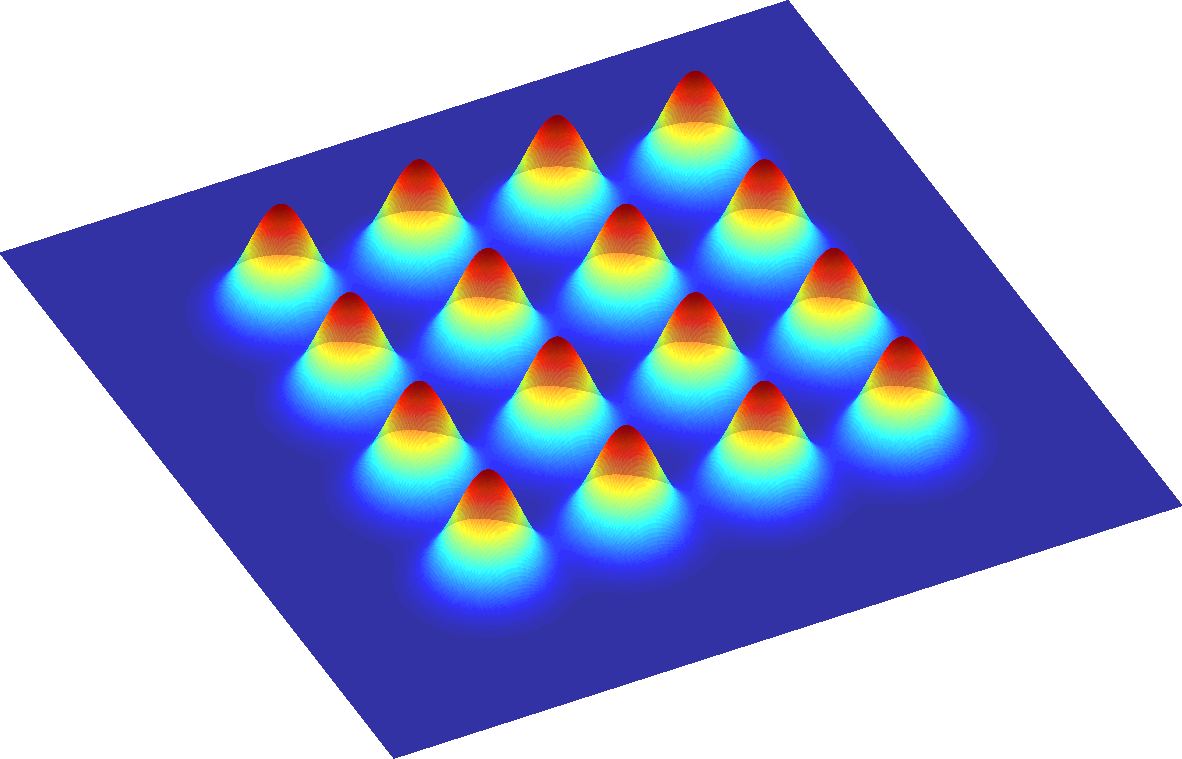
\includegraphics[width=\textwidth]{img/cellLayoutSquare.png}
        \caption{}
        \label{fig:cellLayoutSquare}
    \end{subfigure}
	\begin{subfigure}[t]{0.49\textwidth}
        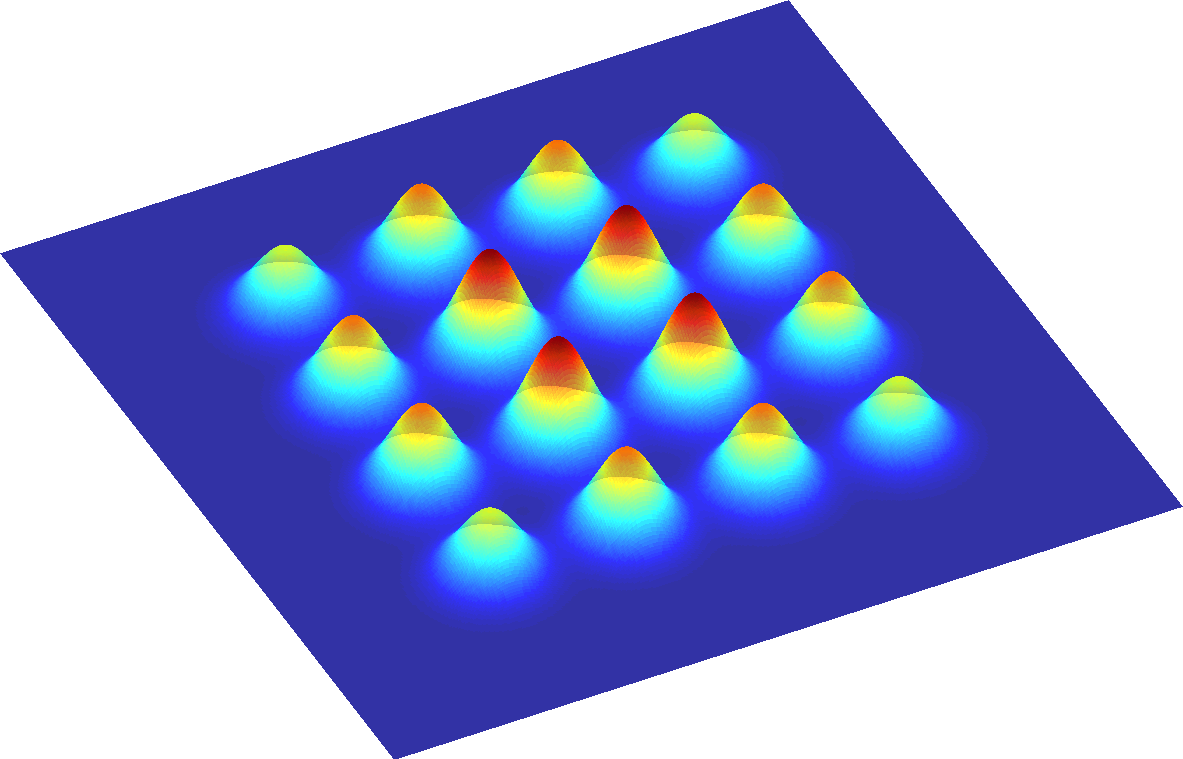
\includegraphics[width=\textwidth]{img/cellLayoutSquareCenter.png}
        \caption{}
        \label{fig:cellLayoutSquareCenter}
    \end{subfigure}
	\begin{subfigure}[t]{0.49\textwidth}
        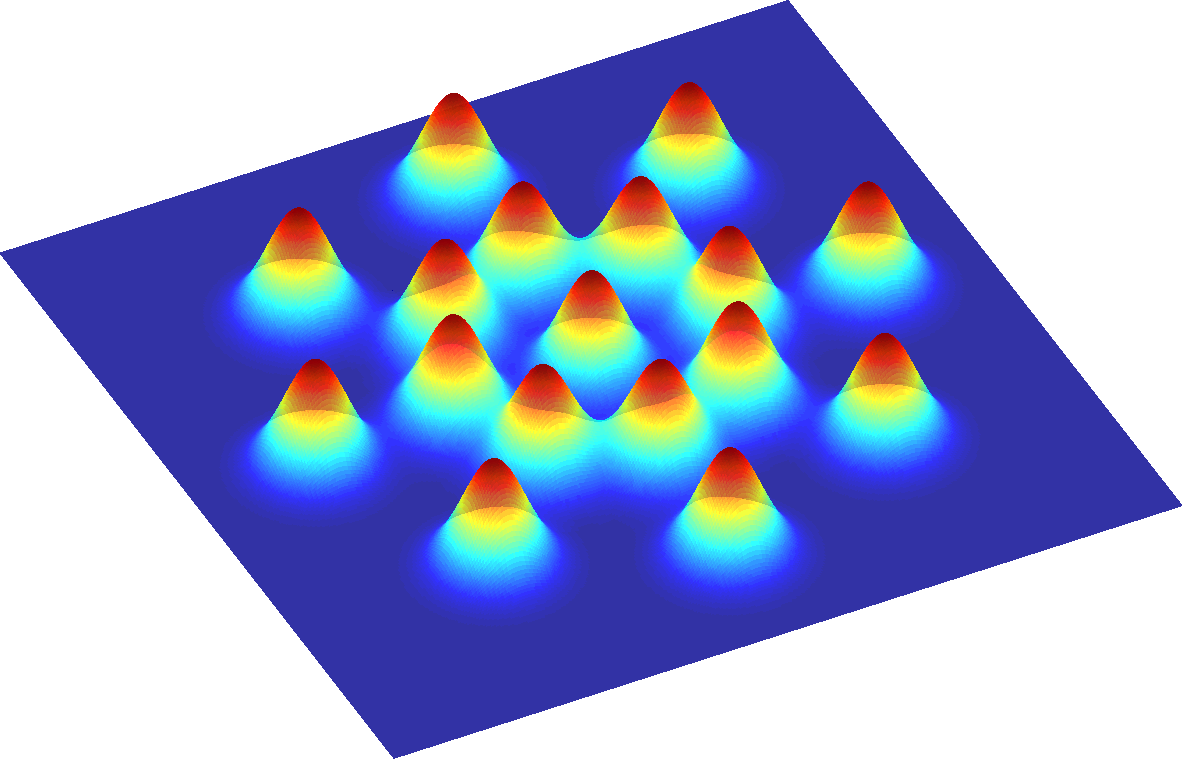
\includegraphics[width=\textwidth]{img/cellLayoutPolar.png}
        \caption{}
        \label{fig:cellLayoutPolar}
    \end{subfigure}
	\begin{subfigure}[t]{0.49\textwidth}
        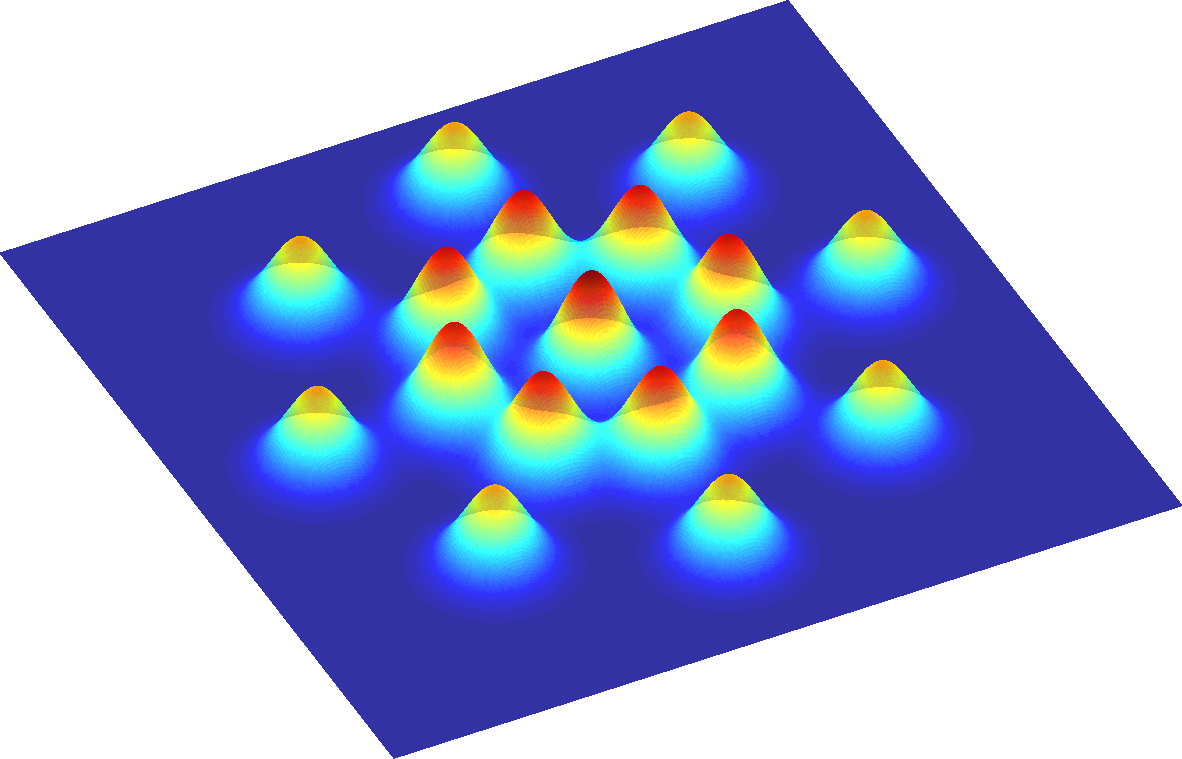
\includegraphics[width=\textwidth]{img/cellLayoutPolarCenter.png}
        \caption{}
        \label{fig:cellLayoutPolarCenter}
    \end{subfigure}
	\begin{subfigure}[t]{0.49\textwidth}
        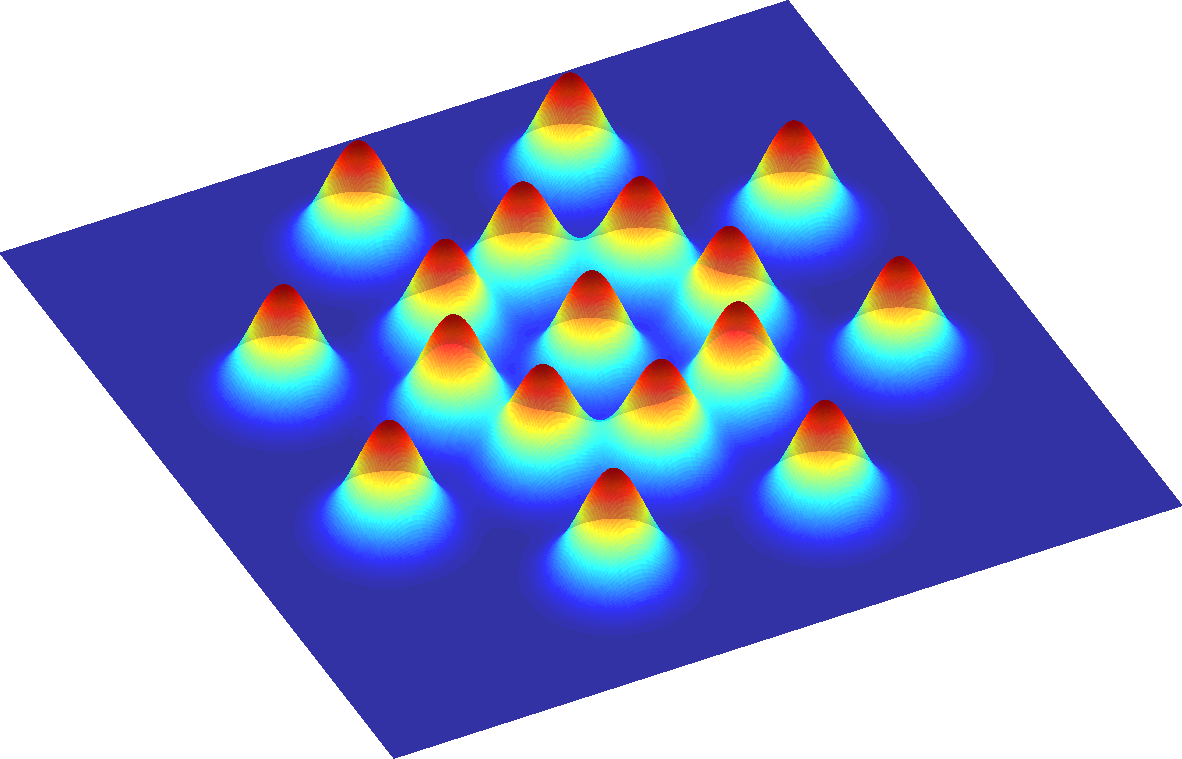
\includegraphics[width=\textwidth]{img/cellLayoutConcentricPolar.png}
        \caption{}
        \label{fig:cellLayoutConcentricPolar}
    \end{subfigure}
	\begin{subfigure}[t]{0.49\textwidth}
        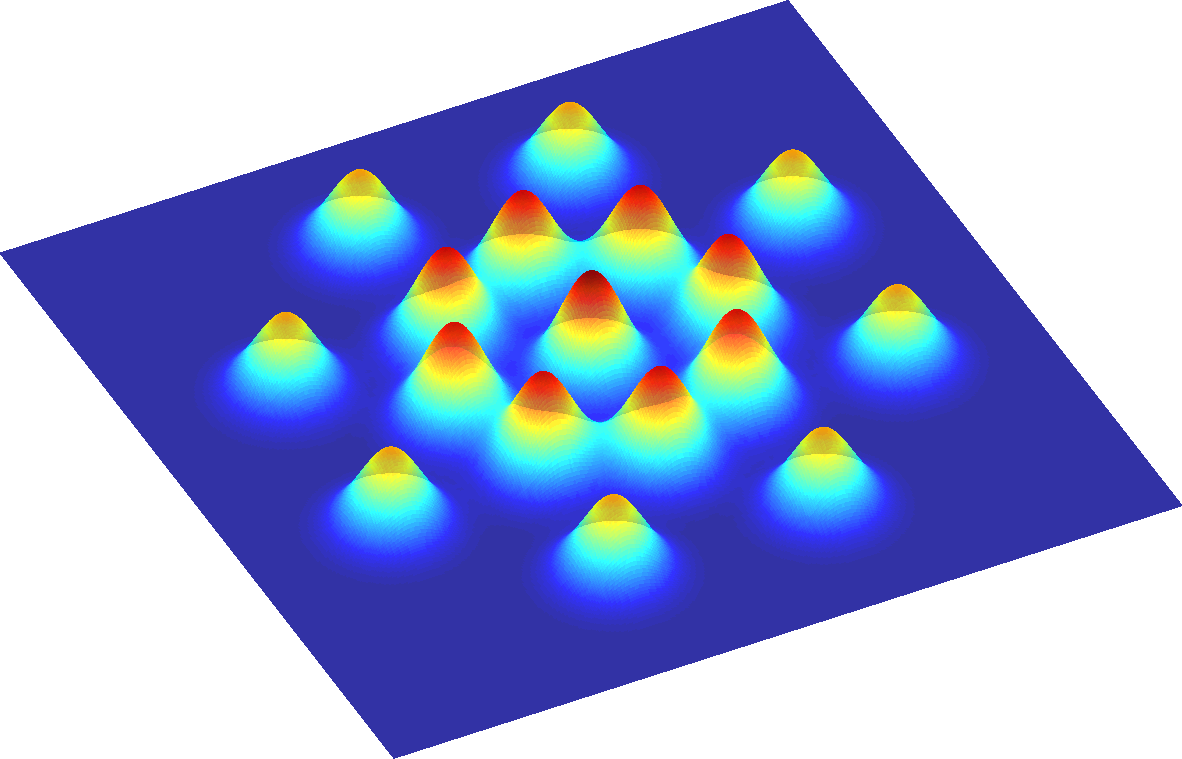
\includegraphics[width=\textwidth]{img/cellLayoutConcentricPolarCenter.png}
        \caption{}
        \label{fig:cellLayoutConcentricPolarCenter}
    \end{subfigure}
    \caption{}
\end{figure}
%
\begin{figure}[H]
    \centering
    \begin{subfigure}[t]{0.49\textwidth}
        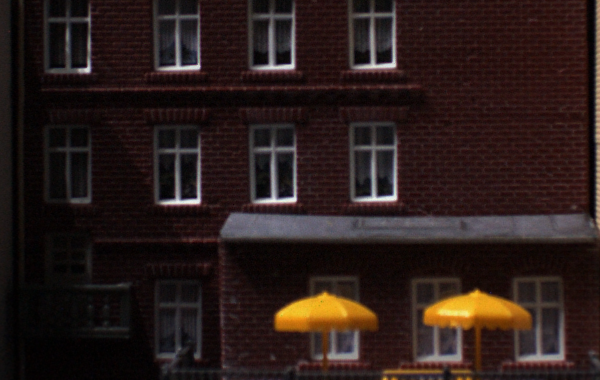
\includegraphics[width=\textwidth]{img/pixelNormalizationExample1.png}
        \caption{}
        \label{fig:pixelNormalizationExample1}
    \end{subfigure}
    \begin{subfigure}[t]{0.49\textwidth}
        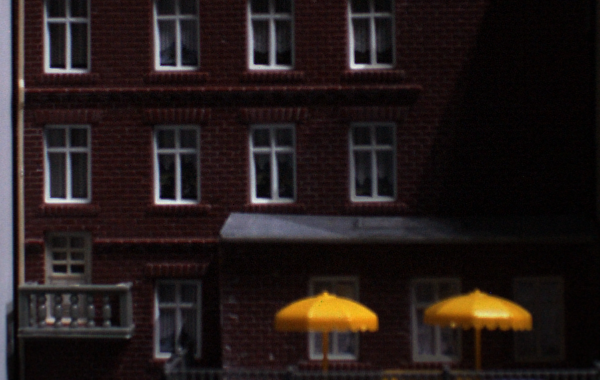
\includegraphics[width=\textwidth]{img/pixelNormalizationExample2.png}
        \caption{}
        \label{fig:pixelNormalizationExample2}
    \end{subfigure}
    \begin{subfigure}[t]{0.49\textwidth}
        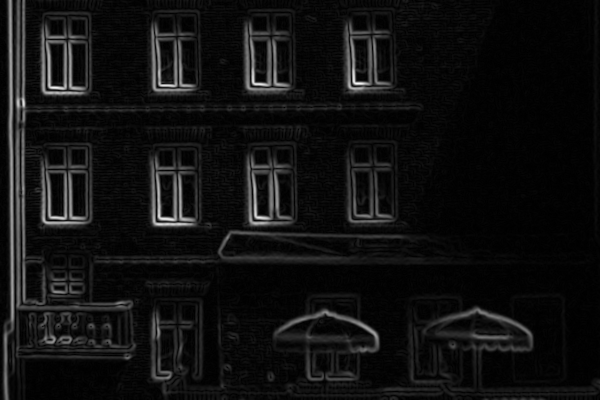
\includegraphics[width=\textwidth]{img/pixelNormalizationExample3.png}
        \caption{}
        \label{fig:pixelNormalizationExample3}
    \end{subfigure}
    \begin{subfigure}[t]{0.49\textwidth}
        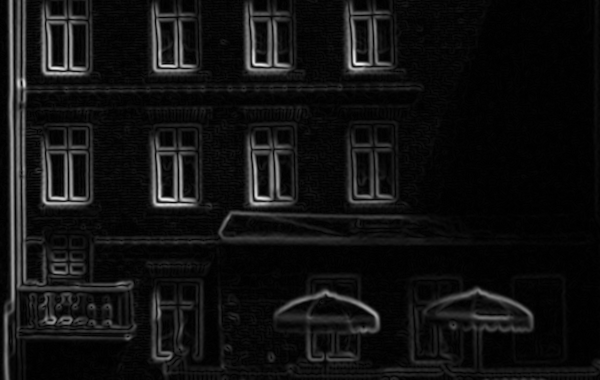
\includegraphics[width=\textwidth]{img/pixelNormalizationExample4.png}
        \caption{}
        \label{fig:pixelNormalizationExample4}
    \end{subfigure}
    \begin{subfigure}[t]{0.49\textwidth}
        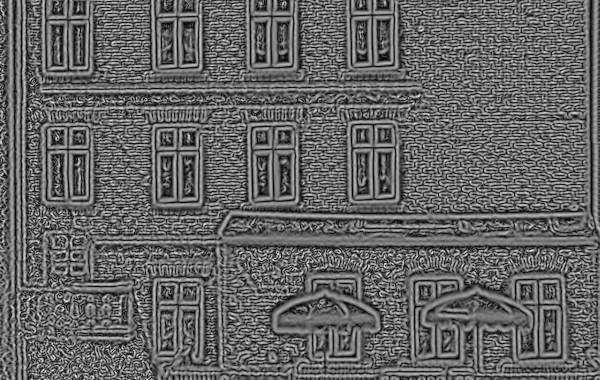
\includegraphics[width=\textwidth]{img/pixelNormalizationExample5.png}
        \caption{}
        \label{fig:pixelNormalizationExample5}
    \end{subfigure}
    \begin{subfigure}[t]{0.49\textwidth}
        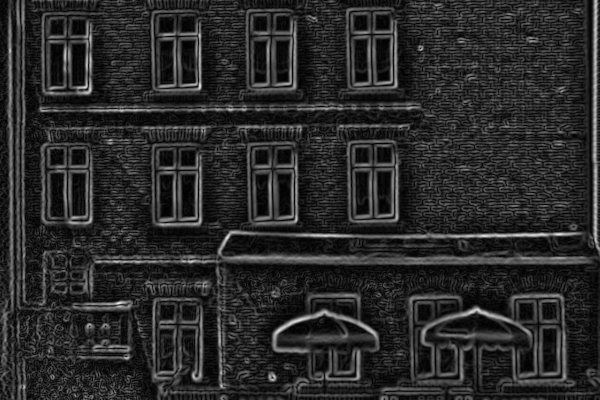
\includegraphics[width=\textwidth]{img/pixelNormalizationExample6.png}
        \caption{}
        \label{fig:pixelNormalizationExample6}
    \end{subfigure}
    \begin{subfigure}[t]{0.49\textwidth}
        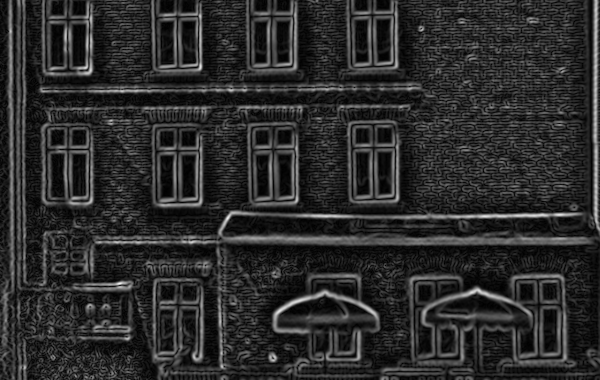
\includegraphics[width=\textwidth]{img/pixelNormalizationExample7.png}
        \caption{}
        \label{fig:pixelNormalizationExample7}
    \end{subfigure}
    \begin{subfigure}[t]{0.49\textwidth}
        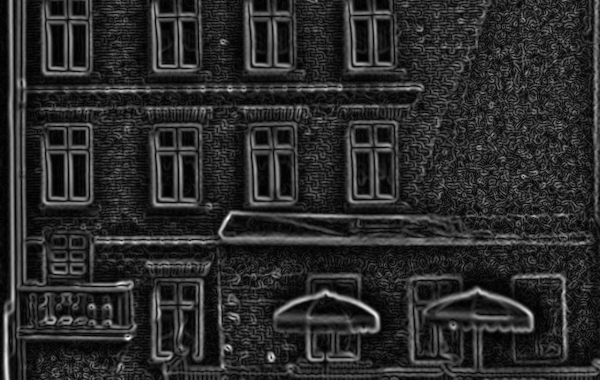
\includegraphics[width=\textwidth]{img/pixelNormalizationExample8.png}
        \caption{}
        \label{fig:pixelNormalizationExample8}
    \end{subfigure}
    \caption{Images \subref{fig:pixelNormalizationExample1} and \subref{fig:pixelNormalizationExample2} show cut-outs of an image with leftmost and rightmost artificial lighting, respectively. Images \subref{fig:pixelNormalizationExample3} and \subref{fig:pixelNormalizationExample4} show gradient magnitudes of these images. Images \subref{fig:pixelNormalizationExample5} and \subref{fig:pixelNormalizationExample6} show pixel normalized magnitudes for $\sigma_\text{norm} = 2$. Images \subref{fig:pixelNormalizationExample7} and \subref{fig:pixelNormalizationExample8} show pixel normalized magnitudes for $\sigma_\text{norm} = 10$.}
    \label{fig:pixelNormalizationExample}
\end{figure}
%
\subsection{Histogram normalization}

- No cell normalization -> Center (cell)

0. Center (pixels) -> no normalization
1. Center (pixels) -> cell normalization
2. Center (pixels) -> Cell normalization -> Center (cell)
3. Cell normalization -> Center (cell)

Center (cell)


\subbibliography

\end{document}
